% Preamble
\documentclass[DIV=13]{scrartcl}

% Packages
\usepackage[T1]{fontenc}
\usepackage[utf8]{inputenc}
\usepackage[english]{babel}
\usepackage{amsmath}
\usepackage{amssymb}
\usepackage{booktabs}
\usepackage{siunitx}
\usepackage{tabu}
\usepackage{graphicx}
\usepackage[expansion=false]{microtype}
\usepackage[sorting=none, maxbibnames=99, maxcitenames=2,backend=biber]{biblatex}
\usepackage{subcaption}
\usepackage[hidelinks]{hyperref}
\usepackage{csquotes}

%\usepackage[newfloat]{minted}
%\usemintedstyle{friendly}
%\setminted{
%    fontsize={\small}
%}

\addbibresource{refs.bib}
\usepackage{symbols}

% Document
\begin{document}
    \title{Rolling Process Variation Estimation Using a Monte-Carlo Method}
    \date{\today}
    \author{
        M. Weiner \thanks{Corresponding author}
        \and
        C. Renzing
%        \and
%        M. Stirl
        \and
        M. Schmidtchen
        \and
        U. Prahl
    }

    \extratitle{
        \minisec{Max Weiner}
        max.weiner@imf.tu-freiberg.de\\
        Conceptualization, Methodology, Software, Formal analysis, Validation, Investigation, Writing - Original Draft\\
        Institute of Metals Forming, TU Bergakademie Freiberg

        \minisec{Christoph Renzing}
        christoph.renzing@imf.tu-freiberg.de\\
        Conceptualization, Methodology, Software, Formal analysis, Validation, Investigation, Project administration, Writing - Original Draft\\
        Institute of Metals Forming, TU Bergakademie Freiberg

%        \minisec{Max Stirl}
%        max.stirl@imf.tu-freiberg.de\\
%        Writing - Review \& Editing\\
%        Institute of Metals Forming, TU Bergakademie Freiberg

        \minisec{Matthias Schmidtchen}
        matthias.schmidtchen@imf.tu-freiberg.de\\
        Conceptualization, Supervision, Resources, Project administration, Writing - Review \& Editing\\
        Institute of Metals Forming, TU Bergakademie Freiberg

        \minisec{Ulrich Prahl}
        ulrich.prahl@imf.tu-freiberg.de\\
        Supervision, Resources, Writing - Review \& Editing\\
        Institute of Metals Forming, TU Bergakademie Freiberg

        \vfill

        \minisec{Funding}
        Not applicable.

        \minisec{Data Availability}
        Data openly available in a public repository that does not issue DOIs.
        Source code and data are available on GitHub at the following URLs:
        \begin{description}
            \item[Project Home] \url{https://github.com/pyroll-project}
            \item[Core Package] \url{https://github.com/pyroll-project/pyroll-core}
            \item[Benchmark Input and Data] \url{https://github.com/pyroll-project/pyroll-pub1-benchmark}
        \end{description}

        \minisec{Conflicts of Interest}
        The authors declare no conflicts of interest.

        \minisec{Acknowledgements}
        The authors thank Richard Pfeifer and Lukas Göschel for the preparation of the data.

        \minisec{Keywords}
        Rolling Simulation; Open Source; Groove Rolling
    }

    \maketitle

    \begin{abstract}

    \end{abstract}


    \section{Introduction}\label{sec:introduction}

    All technical processes are subject to certain variations.
Knowledge and control of these variations is crucial for process stability and product quality.
Sources of variations in a process are the variations already present in the input workpiece and newly generated variations due to imperfections of the process itself.
In the case of wire and bar hot rolling industry regarded here, not only the product geometry, but also the final material properties sre highly sensitiv to the process conditions.
Especially the temperature evolution of the workpiece within the rolling line has high impact on the microstructural transformation processes happening before, during and after forming.
The product's microstructural state determines the mechanical properties and therefore its behavior in further processing and application.
Current alloy concepts in the steel industry increase this problem, as the process window gets more narrow to achieve the property requirements for high-tech applications.
The controlled combination of forming and thermally activated material transformation is commonly subsumed under the term thermo-mechanical treatment.

The classic way of analysing variational behavior with mathematical tooling is the error propagation using first order Taylor series expansions (see f.e.~\cite{Ku1966}).
This concept is widely used in science and industry, especially to determine the error of indirect measurement processes.
This procedure has two main problems.
First, one needs to determine the first derivatives of the regarded function in each dimension, either analytically or numerically, which is rather problematic if the function is complicated.
Second, the error is commonly represented in terms of the variance, so there is only information about the spread, but not about the shape of the distribution inherent.

The usage of a Monte-Carlo Method circumvents these problems, and shall be proposed with this work.
The term Monte Carlo Method (MCM) generally refers to a class of methods, which are characterized by the use of random numbers.
These methods are rather diverse and serve different purposes.
Here, the term shall be used for the concept of drawing random numbers as input for a function and analysing the results of several evaluations of this function, with different random inputs, with statistical methods.
A detailed overview on this type of Monte Carlo methods is given by \textcite{Lemieux2009}.
The nature of the function can be complicated, even of a black-box type, where nothing about the internals of the function is known but the input and output interfaces.
In this case, Monte Carlo methods can provide valuable information about the behavior of the function while altering inputs.
Also, the complete distribution of the input variables is included in the estimation and is reflected in the results.

Here, the function equals the simulation procedure, so it is generally known, but complicated.
For example, it is generally not possible, to compute derivatives of the outputs in dependence on the inputs in an analytical way.
Even numerical derivation is hard, due to the multi-dimensional nature of most natural or technical systems and the pronounced non-linear behavior of the function.

The use of Monte Carlo methods for the analysis of variations in technical processes was reported before in the field of assembly of complicated structures, like in mechanical engineering and building construction (f.e.~\cite{Lin1997, Shen2005, Dantan2009, Qureshi2012, Yan2015, Rausch2019}).
However, in the field of rolling processes, there was no such attempt yet to the knowledge of the authors.
The authors have previously used a similar approach to model powder morphology influences in sintering processes~\cite{Weiner2022, Weiner2022b}.
The current work shall show the possibility of the application of Monte Carlo methods for the analysis of process variations in rolling processes.
The focus lies hereby on the estimation of the workpiece temperature evolution and its impact on the microstructure state of the final product.
The influence of variations in the initial workpiece and within the regarded process route is analysed and evaluated.
Due to the need of a large number of function evaluations (simulation runs), the evaluation speed of the process model is crucial to the applicability of this approach.

Rolling simulation is currently dominated by the use of finite element (FE) based models.
These are offering high accuracy and high resolution results at the expense of high computational resource usage.
So these methods are inconvenient for the current need.
Therefore, one-dimensional approaches shall be used here.
These offer less accuracy and limited resolution, but are computable within fractions of seconds on typical personal computer systems.
The current work is based on the open-source rolling simulation framework PyRolL~\cite{pyroll2}, developed by the authors, which is a fast, open and flexible software package mainly aimed at groove rolling in reduction passes.
The models used for the different parts of the problem can be exchanged and extended with low effort to the users needs.




    \section{Methods}\label{sec:methods}

    \subsection{Experimental Procedure}\label{subsec:experimental-procedure}

The object of the current investigation is the operation of the experimental semi-continuous rolling plant located at the Institute of Metal Forming, TU Bergakademie Freiberg.
It consists of a two-high reversing roughing stand and four continuous finishing stands.
The pass schedule of the current work consists of 10 oval-round reversing passes (R1-10) followed by 4 oval-round continuous finishing passes (F1-4).
A \qty{50}{\milli\meter} round workpiece made of C45 carbon steel is rolled down to \qty{8}{\milli\meter} diameter, starting at \qty{1150}{\celsius}, resp.\ \qty{1423.15}{\kelvin}.
Details of the schedule are provided in \autoref{tab:process_conditions} and in the supplemental material~\cite{WeinerVariationSupplemental2024}.
The profile shapes appearing in the schedule are illustrated in \autoref{fig:plot_pass_sequence}.

\begin{figure}
    \centering
    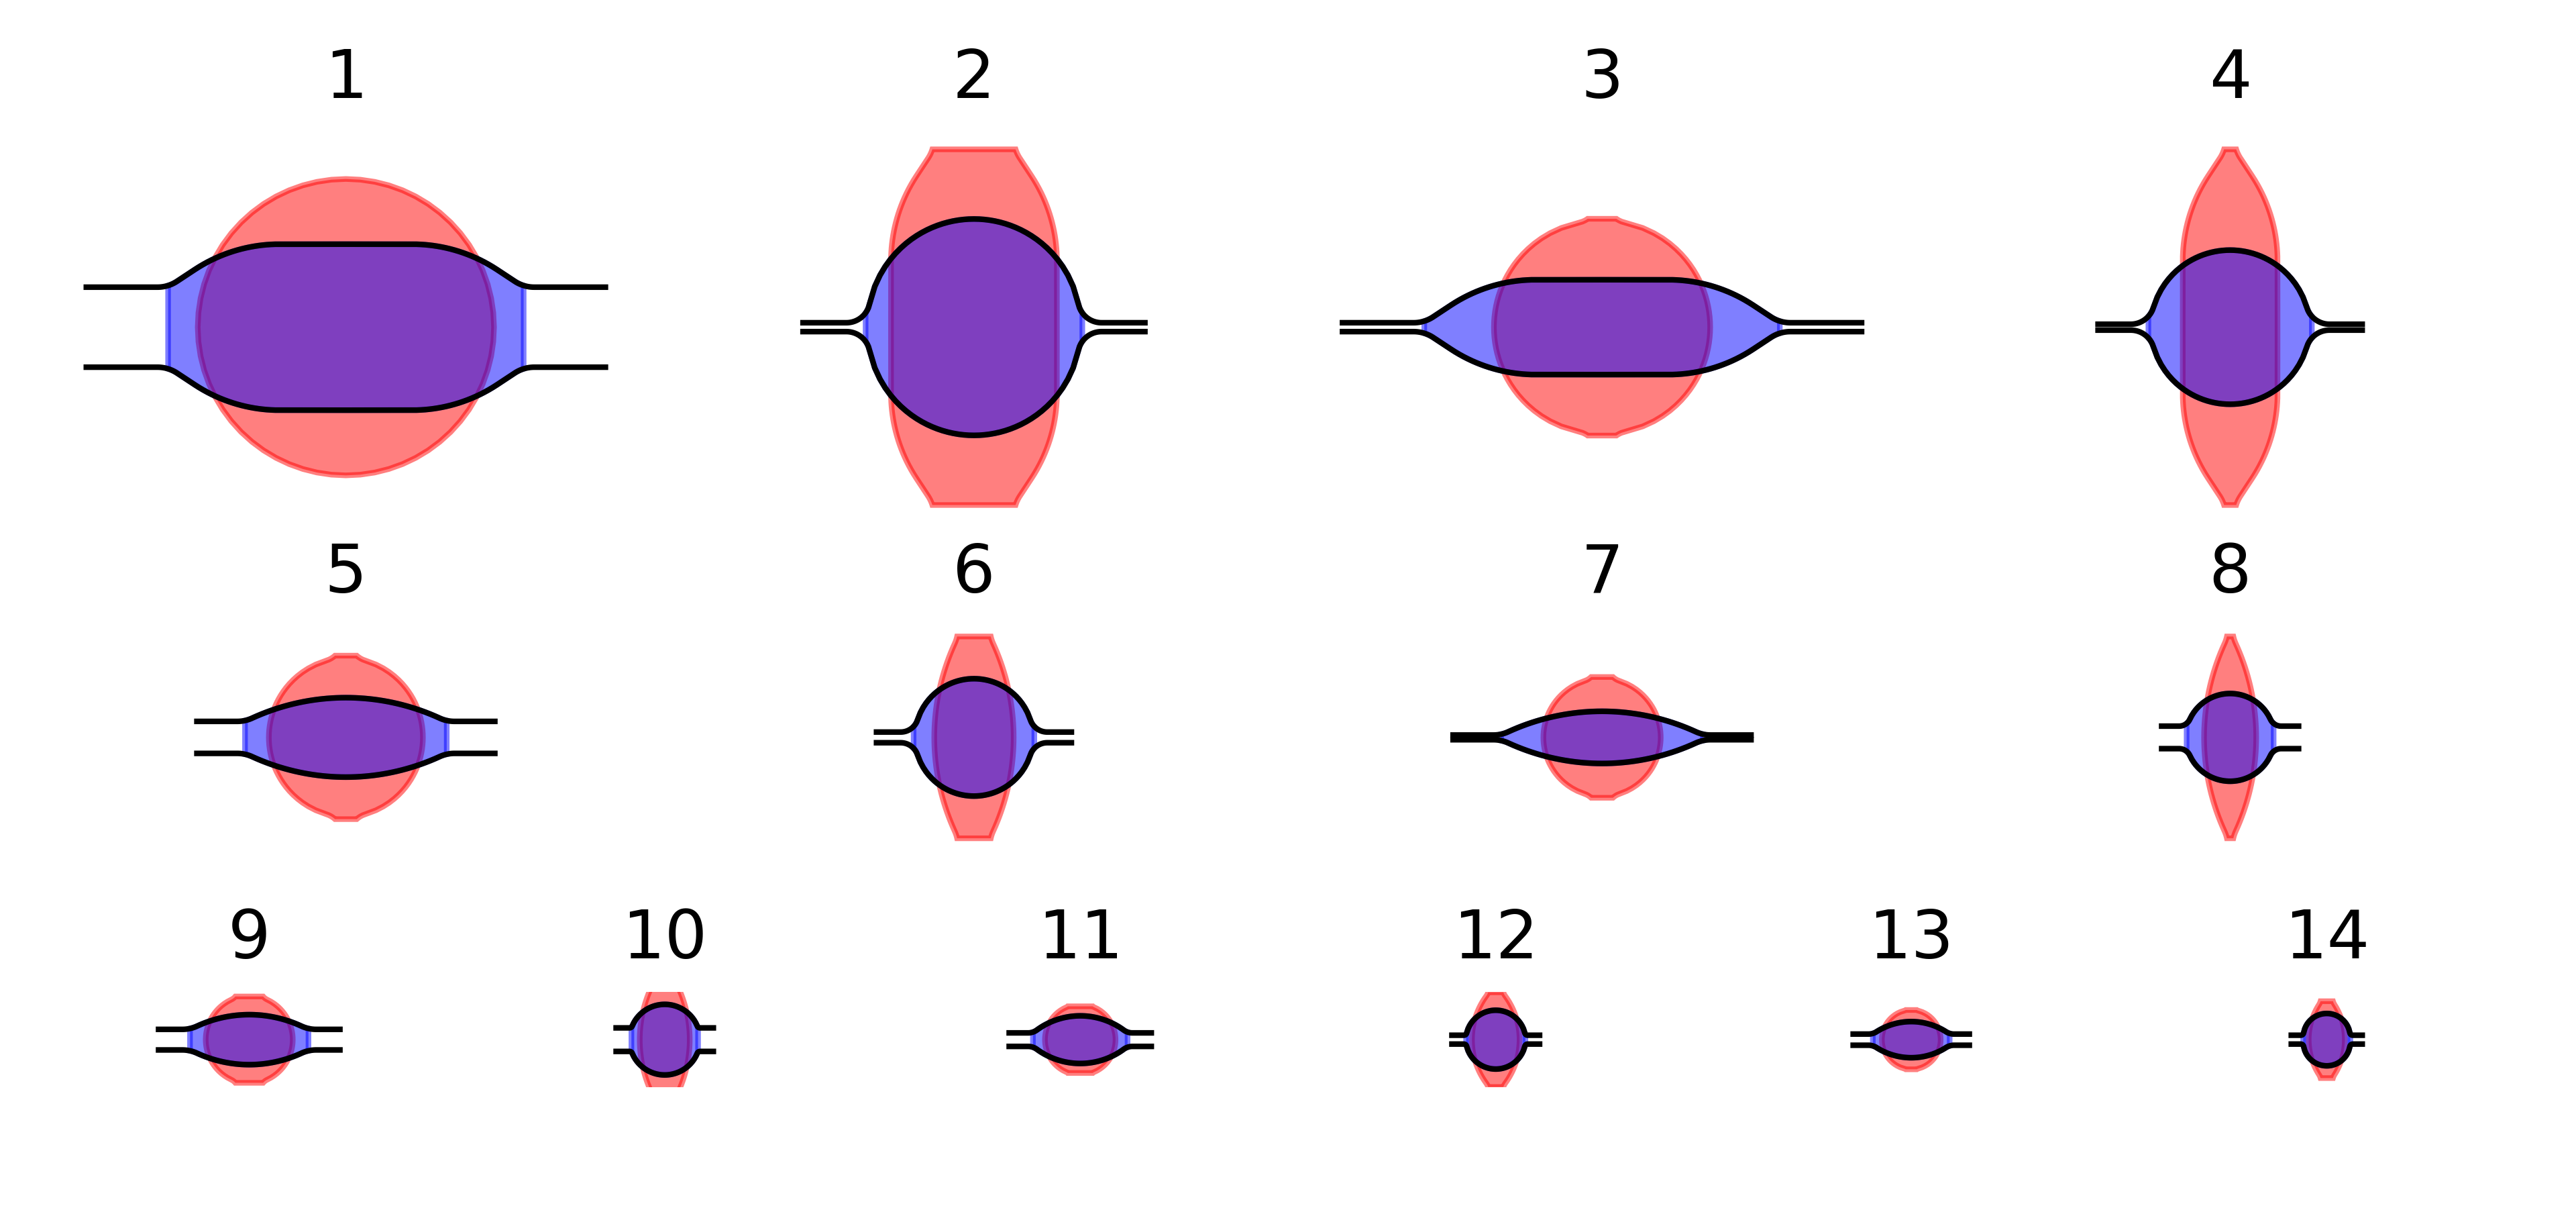
\includegraphics{img/plot_pass_sequence}
    \caption{True Scaled Illustration of the Investigated Pass Sequence}
    \label{fig:plot_pass_sequence}
\end{figure}


\begin{table}
    \centering
    \caption{Principal Data of the Investigated Pass Sequence}
    \label{tab:process_conditions}
    \begin{tblr}{colspec={l|XXXXXX}}
    \toprule
    \#             & Type                       & $\Width$                                               & $\Height$                                              & $\RollGap$                              & $\RollRadius$                                           & $\Velocity$                          \\
    &                            & \unit{\milli\meter}                                    & \unit{\milli\meter}                                    & \unit{\milli\meter}                     & \unit{\milli\meter}     & \unit{\meter\per\second}   \\
    \midrule
    
    {{ p.label }} & {{ p | format_pass_type }} & \num{ {{- (p.out_profile.width * 1e3) | round(1) -}} } & \num{ {{-  (p.out_profile.height * 1e3) | round(1) -}} } & \num{ {{-  (p.gap * 1e3) | round(1) -}} } & \num{ {{-  (p.roll.nominal_radius * 1e3) | round(1) -}} } & \num{ {{-  p.velocity | round(1) -}} }\\
    
    \bottomrule
\end{tblr}
\end{table}

Inline measurements of the process conditions and workpiece state are done regarding roll force and torque, as well as workpiece temperature.
The latter is measured using pyrometers at several points in the plant: at the entry and exit of the reversing stand and before, between and after the finishing stands.
The sensor signals are collected as timelines, so that they can be automatically analysed afterwards as described in \autoref{subsec:data-acquisition}.

To achieve statistical certainty, 45 rolling trials were carried out.
This enables an estimation of the variations appearing.
A major source of variation in these trials is the manual feeding of the workpiece into the reversing passes.
The duration of those is scheduled with about 6 seconds.
The actual time needed has to be investigated in this work, see \autoref{subsec:data-acquisition} for details.

\subsection{Monte-Carlo Approach}\label{subsec:monte-carlo-approach}

\begin{figure}
    \centering
    \includegraphics[width=\linewidth]{img/chart_mc_principle}
    \caption{Chart of the Concept of Variation Estimation Using Monte Carlo Techniques}
    \label{fig:chart_mc_principle}
\end{figure}

The basic idea of the approach shown here is to simulate the rolling process several times with different input values, which are drawn by a random number generator according to predefined statistical distributions.
Afterwards, the distribution of the results can be analysed by classic methods of descriptive statistics to obtain information about the process' variational behavior.
The principle is shown in \autoref{fig:chart_mc_principle}.

This approach provides information about the overall variational behavior of the process.
If a single source of variation is introduced in the input, the reaction of the process on this variable can be analysed.
The count of variation sources that can be introduced is generally unbounded.
In contrast to classic Taylor series error propagation, the computational effort does not directly increase remarkably with increasing count of investigated parameters.
However, an increase in sample size can be necessary to achieve sufficient certainty.
The key problem is to obtain data describing the variations of the input variables.
The tracing back of result variations to the input can be done using classic correlation methods of descriptive statistics, however, with the same typical caveats.
The main benefit of the approach is that no information about the internals of the simulation procedure is needed for variational analysis, especially there is no need for derivatives of result values in dependence on the input.
The simulation procedure can generally be treated as black box with defined input and output interfaces.

\subsection{Statistical Data Acquisition}\label{subsec:data-acquisition}

As input for the Monte-Carlo approach statistical descriptions of the regarded input variables are needed.
Regarding the geometric variations of the input workpiece, the diameter of the samples was determined at multiple spots using a calibre.
The initial temperature of the samples was determined using the pyrometer installed near the roll gap entry.
Both were approximated using a normal distribution for sampling of random input values.

The question of varying inter-pass durations is crucial for scientific experiments on microstructure evolution, but currently often neglected.
Mostly, only fixed durations between the reversing passes are included in the design calculations.
Due to manual transport and feed of the workpiece to the following roll pass, the scheduled inter-pass durations are never realized in practice.
Nevertheless, these deviations from the schedule influence the microstructure evolution of the sample, as well as the actual conditions in the roll passes.
The current approach is aimed to help quantifying these deviations.

To obtain the inter-pass durations $\Pause{\Duration}$ from the timeline data, the passes have to be identified automatically.
This was done by analysing the roll torque signal as plotted in \autoref{fig:plot_timeline_pass_finding}.
The original signal was first downsampled and smoothed.
Then, a difference filter was applied and the peaks of the resulting signal were determined.
These peaks denote start and end times of the roll passes, the middle time of those was used as time coordinate of the roll pass.
The distances of those were used as the inter-pass durations.

\begin{figure}
    \centering
    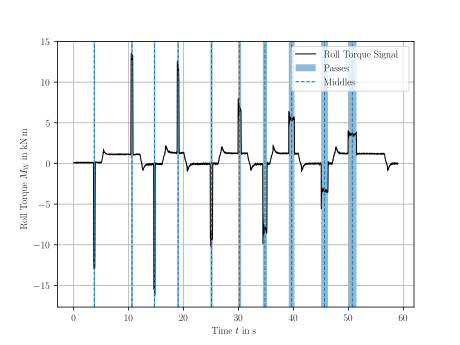
\includegraphics{img/plot_timeline_pass_finding}
    \caption{Example Roll Torque Signal With Automatically Determined Roll Pass Locations}
    \label{fig:plot_timeline_pass_finding}
\end{figure}

For the approximative description of the durations' distribution, a Weibull distribution was used.
The probability density function (PDF) of the Weibull distribution is defined as in \autoref{eq:weibull-dist},
where $\WeibullDistributionShape > 0$ and $\WeibullDistributionScale > 0$ are the shape and scale parameters.
The distribution function was fitted on the observed data using the least-squares method.

\begin{equation}
    p\left(\Pause\Duration \right)=\frac{\WeibullDistributionShape}{\WeibullDistributionScale} \left(\frac{\Pause\Duration}{\WeibullDistributionScale}\right)^{\WeibullDistributionShape-1}\exp -\left(\frac{\Pause{\Duration}}{\WeibullDistributionScale} \right)^{\WeibullDistributionShape}
    \label{eq:weibull-dist}
\end{equation}

\subsection{Core Simulation Procedure}\label{subsec:simulation-procedure}

In the current work, the open-source rolling simulation framework PyRolL~\cite{pyroll_jors, pyroll2.1} was used to simulate the rolling process.
Generally, the shown approach can be used with every rolling simulation software available, since the procedure does not depend on any internals of the simulation.
A fast simulation approach, however, is favourable, since the simulation has to be done several, up to hundreds of, times.
The models used here are of one-dimensional type, thus, they lack of resolution in other directions as the rolling direction and provide only limited accuracy, but at the benefit of high solution speed.
They typically combine empirical approaches with simplified analytical solutions.
The simulation was done with the basic configuration of PyRolL, which includes the empirical roll force and torque model of \textcite{Hensel1978}, an integral thermal model approach according to \textcite{Hensel1990}, contact area estimation according to \textcite{Zouhar1960} and roll flattening according to \textcite{Hitchcock1935}.
Spreading was simulated using the equivalent flat pass according to \citeauthor*{Lendl1948}~\cite{Lendl1948, Lendl1948a, Lendl1949} in conjunction with the spreading equation of \textcite{Wusatowski1969}.
Details of software construction and model equations are provided in the documentation of PyRolL~\cite{pyroll}.


The models most important for the following elaborations will be discussed in brief.
The temperature change of the workpiece was calculated by an integral heat balance as proposed by \textcite{Hensel1990} and given in \autoref{eq:heat-balance}.

\begin{equation}
    \Delta\Temperature = \Convection{\Delta\Temperature} + \Contact{\Delta\Temperature} + \Delta\Temperature_\Deformation + \Radiation{\Delta\Temperature}
    \label{eq:heat-balance}
\end{equation}

\noindent$\Convection{\Delta\Temperature}$ is the temperature change by convective heat flows according to \autoref{eq:heat-convection} with $\Convection{\HeatTransferFactor}$ as a heat transfer factor, $\Environment{\Temperature}$ as the environment temperature, $\Temperature$ as the current workpiece temperature and $\Duration$ as the duration of the process step.

\begin{equation}
    \Convection{\Delta\Temperature} = \frac{\Convection{\HeatTransferFactor} \Surface\Area}{\Density\ThermalCapacity\Volume} \left( \Environment{\Temperature} - \Temperature \right) \Duration
    \label{eq:heat-convection}
\end{equation}

\noindent$\Contact{\Delta\Temperature}$ is the temperature change by contact to the rolls according to \autoref{eq:heat-contact} with $\Contact{\HeatTransferFactor}$ as a heat transfer factor and $\Roll{\Temperature}$ as the temperature of the rolls.

\begin{equation}
    \Contact{\Delta\Temperature} = \frac{\Contact{\HeatTransferFactor} \Contact\Area}{\Density\ThermalCapacity\Volume} \left( \Roll{\Temperature} - \Temperature \right) \Duration
    \label{eq:heat-contact}
\end{equation}

\noindent$\Radiation{\Delta\Temperature}$ is the temperature change by radiation according to \autoref{eq:heat-radiation} with $\StefanBoltzmannCoefficient$ as the Stefan's and Boltzmann's constant and $\RelativeRadiationCoefficient$ as the relative radiation coefficient of the gray radiator.

\begin{equation}
    \Radiation{\Delta\Temperature} = \frac{\StefanBoltzmannCoefficient \RelativeRadiationCoefficient \Surface\Area}{\Density\ThermalCapacity\Volume} \left( \Environment{\Temperature}^4 - \Temperature^4 \right) \Duration
    \label{eq:heat-radiation}
\end{equation}

\noindent$\Delta\Temperature_\Deformation$ is the temperature change by deformation according to \autoref{eq:heat-deformation} with $\DeformationResistance$ as the empirical deformation resistance and $\Equivalent\LogStrain$ as the equivalent plastic strain.
Since the deformation resistance is used here instead of the flow stress, this term also includes approximately the heat generation by inner and outer friction.

\begin{equation}
    \Delta\Temperature_\Deformation = \frac{\num{0.95} \DeformationResistance \Equivalent\LogStrain}{\Density\ThermalCapacity}
    \label{eq:heat-deformation}
\end{equation}

The deformation resistance was taken as proposed by \textcite{Hensel1978} and given in \autoref{eq:deformation-resistance}.

\begin{multline}
    \frac{\DeformationResistance}{\Equivalent\FlowStress} = \num{0.9901} + \num{0.106} \frac{\Contact\Area}{\Equivalent\CrossSection} + \num{0.0283} \left( \frac{\Contact\Area}{\Equivalent\CrossSection} \right)^2 + \num{1.5718} \exp \left[ \num{-2.4609} \frac{\Contact\Area}{\Equivalent\CrossSection} \right] \\
    + \num{0.3117} \exp \left[ \num{-15.625} \left( \frac{\Contact\Area}{\Equivalent\CrossSection} \right)^2 \right]
    \label{eq:deformation-resistance}
\end{multline}

To pay regard on the microstructure influence of the thermal variation involved in the process, a JMAK based recrystallization model was used.
The JMAK approach is named after \textcite{Johnson1939}, \textcite{Avrami1939, Avrami1940, Avrami1941} and \textcite{Kolmogorov1937}.
It has gained a large popularity in modelling kinetics of transformation processes.
The literature regarding recrystallization modelled by JMAK approaches is rather diverse~\cite{Luton1969, Sellars1978, Sellars1979, Sellars1985, Beynon1992, Glover1972, Glover1973, Hodgson1992, Laasraoui1991, Laasraoui1991a, Hernandez1996, Medina1996, Fernandez2000, Fernandez2003, Karhausen1992,Roberts1979, Maccagno1996, Siciliano2000}.
There are many forms of how the parameters can be described for materials under different conditions regarding strain $\LogStrain$, strain rate $\LogStrainRate$ and temperature $\Temperature$.
The following equations try to generalize them into one for all three major mechanisms: dynamic, metadynamic and static recrystallization.
The Zener-Holomon-parameter~\cite{Zener1944} is not applied here, since sometimes different activation energies are used therein for the distinct mechanisms, so the Arrhenius-term is explicitly used in each equation.
These equations are implemented in the JMAK Recrystallization Plugin for PyRolL~\cite{pyroll-jmak-recrystallization}.

The recrystallized fraction $\RecrystallizedFraction$ in dependence on time $\Time$ is given as Avrami-term as \autoref{eq:jmak-fraction}, with the empirical parameters $k$ an $n$, as well as the reference time $\Time_\Reference$ and critical time $\Time_{\Critical}$.

\begin{equation}
    \RecrystallizedFraction(\Time) = 1 - \exp \left[ k \left( \frac{\Time - \Time_\Critical}{\Time_\Reference - \Time_\Critical} \right)^n \right]
    \label{eq:jmak-fraction}
\end{equation}

The critical time $\Time_\Critical$ is the incubation time of the recrystallization, thus the time, when the recrystallization starts.
It is calculated by an empirical approach according to \autoref{eq:jmak-critical} with the material dependent parameters $a_i$ and the activation energy $\ActivationEnergy_a$.

\begin{equation}
    \Time_{\Critical} = a_1 \cdot \LogStrain_{\In}^{a_2} \cdot \LogStrainRate^{a_3} \cdot \GrainSize_{\In}^{a_4} \cdot \exp \left[ \frac{\ActivationEnergy_a}{\GasConstant \Temperature} \right]
    \label{eq:jmak-critical}
\end{equation}

The reference time $\Time_\Reference$ is often chosen as the time of half recrystallization $\Time_{0.5}$, then $k$ in \autoref{eq:jmak-fraction} equals $\ln \frac12$.
It is calculated by an empirical approach according to \autoref{eq:jmak-reference} with the material dependent parameters $b_i$ and the activation energy $\ActivationEnergy_b$.

\begin{equation}
    \Time_{\Reference} = b_1 \cdot \LogStrain_{\In}^{b_2} \cdot \LogStrainRate^{b_3} \cdot \GrainSize_{\In}^{b_4} \cdot \exp \left[ \frac{\ActivationEnergy_b}{\GasConstant \Temperature} \right]
    \label{eq:jmak-reference}
\end{equation}

The grain size $\GrainSize_{\mathrm{RX}}$ of the newly recrystallized grains is given by a similar approach according to \autoref{eq:jmak-grain-size} with the material-dependent parameters $c_i$ and the activation energy $\ActivationEnergy_c$.

\begin{equation}
    \GrainSize_{\mathrm{RX}} = c_1 \cdot \LogStrain_{\In}^{c_2} \cdot \LogStrainRate^{c_3} \cdot \GrainSize_{\In}^{c_4} \cdot \exp \left[ \frac{\ActivationEnergy_c}{\GasConstant \Temperature} \right]
    \label{eq:jmak-grain-size}
\end{equation}

These equations include all approaches found in the cited references for static, dynamic and metadynamic recrystallization.
Parameters can be set to zero, if the respective dependency is not needed or not investigated.
For dynamic recrystallization, the time $\Time$ if often substituted by the logarithmic strain $\LogStrain$ under the assumption of constant strain rate, where the same empirical approaches are applied.

The material data and model coefficients used above were taken for the following simulations as in \autoref{tab:material_data}.

\begin{table}
    \centering
    \caption{Material Data and Model Coefficients Used in the Simulations}
    \label{tab:material_data}
    \begin{subtable}{\linewidth}
    \caption{Flow Stress Model of C45 acc.~to~\cite{Spittel2009}}
    \begin{tblr}{
        colspec={XXXXX},
        columns={r},
        row{1}={1cm,m},
        row{2}={l},
        row{4}={l},
        cell{1}{1} = {c=7}{c},
        cell{4-5}{4,6} = {c=2}{},
    }
        \toprule
        $\displaystyle \FlowStress = \FlowStressA \cdot \E^{\FlowStressM1 \CelsiusTemperature} \cdot \LogStrain^{\FlowStressM2} \cdot \LogStrainRate^{\FlowStressM3} \cdot \E^{\FlowStressM4/\LogStrain} \cdot \left( 1 + \LogStrain \right)^{\FlowStressM5\CelsiusTemperature + \FlowStressM6} \cdot \E^{\FlowStressM7\LogStrain} \cdot \left( 1 + \LogStrainRate \right)^{\FlowStressM8\CelsiusTemperature} \cdot \CelsiusTemperature^{\FlowStressM9}$ \\
        $\FlowStressA$ & $\FlowStressM{{- i -}}$ \\
            \midrule
            \num{ {{- c.a / 1e6 -}} } & \num{ {{- c["m{}".format(i)] -}} } \\[3mm]
            $\FlowStressM{{- i -}}$ &  $\CelsiusTemperature$ && $\LogStrain$ \\
            \midrule
            \num{ {{- c["m{}".format(i)] -}} } &  \qtyrange{820}{1200}{\celsius} && \numrange{0.04}{1.5}\\
            \bottomrule
    \end{tblr}
\end{subtable}
\\\vspace{1em}
\begin{subtable}{\linewidth}
    \caption{Parameters for Generalized JMAK Model as in Equations~\ref{eq:jmak-fraction} to~\ref{eq:jmak-grain-size} acc.~to \textcite{Hodgson1992}}
    \begin{tblr}{
        colspec={llXXXX},
        columns={r},
        row{1}={l},
        column{1-2}={l},
    }
        \toprule
        Mechanism & Parameter & 1 & 2 & 3 & 4 \\
        \midrule
        Dynamic
        & $a$ & \num{ {{- "{:.2e}".format(drx.a1) -}} } & \num{ {{- drx.a2 -}} } & \num{ {{- drx.a3 -}} } & \num{ {{- drx.a4 -}} } \\
        & $b$ & \num{ {{- "{:.2e}".format(drx.b1) -}} } & \num{ {{- drx.b2 -}} } & \num{ {{- drx.b3 -}} } & \num{ {{- drx.b4 -}} } \\
        & $c$ & \num{ {{- "{:.2e}".format(drx.c1) -}} } & \num{ {{- drx.c2 -}} } & \num{ {{- drx.c3 -}} } & \num{ {{- drx.c4 -}} } \\
        Meta-Dynamic
        & $a$ & \num{ {{- "{:.2e}".format(mrx.a1) -}} } & \num{ {{- mrx.a2 -}} } & \num{ {{- mrx.a3 -}} } & \num{ {{- mrx.a4 -}} } \\
        & $b$ & \num{ {{- "{:.2e}".format(mrx.b1) -}} } & \num{ {{- mrx.b2 -}} } & \num{ {{- mrx.b3 -}} } & \num{ {{- mrx.b4 -}} } \\
        & $c$ & \num{ {{- "{:.2e}".format(mrx.c1) -}} } & \num{ {{- mrx.c2 -}} } & \num{ {{- mrx.c3 -}} } & \num{ {{- mrx.c4 -}} } \\
        Static
        & $a$ & \num{ {{- "{:.2e}".format(srx.a1) -}} } & \num{ {{- srx.a2 -}} } & \num{ {{- srx.a3 -}} } & \num{ {{- srx.a4 -}} } \\
        & $b$ & \num{ {{- "{:.2e}".format(srx.b1) -}} } & \num{ {{- srx.b2 -}} } & \num{ {{- srx.b3 -}} } & \num{ {{- srx.b4 -}} } \\
        & $c$ & \num{ {{- "{:.2e}".format(srx.c1) -}} } & \num{ {{- srx.c2 -}} } & \num{ {{- srx.c3 -}} } & \num{ {{- srx.c4 -}} } \\
        \bottomrule
    \end{tblr}
\end{subtable}
\\\vspace{1em}
\begin{subtable}{\linewidth}
    \caption{Other Material Data and Model Coefficients}
    \begin{tblr}{
        colspec={XXXXX},
        columns={r},
        row{1-2}={l},
    }
        \toprule
        $\Density$                                  & $\ThermalCapacity$                                   & $\Contact{\HeatTransferFactor}$                        & $\Convection{\HeatTransferFactor}$ & $\RelativeRadiationCoefficient$                    \\
        \unit{\kilo\gram\per\cubic\meter}           & \unit{\joule\per\kilo\gram\per\kelvin}               & \unit{\watt\per\square\meter\per\kelvin} & \unit{\watt\per\square\meter\per\kelvin} & \\
        \midrule
        \num{ {{- "{:.1f}".format(ip.density) -}} } &
        \num{ {{- "{:.1f}".format(ip.specific_heat_capacity) -}} } &
        \num{ {{- "{:.1f}".format(alpha_cont) -}} } &
        \num{ {{- "{:.1f}".format(alpha_conv) -}} }  &
        \num{ {{- "{:.1f}".format(epsr) -}} } \\
        \bottomrule
    \end{tblr}
\end{subtable}

\end{table}




    \section{Results}\label{sec:results}

    \subsection{Analysis of Inter-Pass Durations}\label{subsec:analysis-of-inter-pass-durations}

\begin{figure}
    \centering
    \includegraphics[width=\linewidth]{img/plot_histogram_pauses_all}
    \caption{Density and Cumulative Histograms of Inter-Pass Durations With Fitted Weibull Distributions}
    \label{fig:plot_histogram_pauses}
\end{figure}

\begin{table}
    \centering
    \caption{Descriptive Statistics and Weibull Distribution Parameters of Inter-Pass Durations}
    \label{tab:pause_distributions}
    \begin{tblr}{
    colspec={l|XXXXXX},
    column{2-7}={r},
    row{1-2}={l},
}
    \toprule
    \# & Mean & Std            & Min           & Max            & Shape $\WeibullDistributionShape$ & Scale $\WeibullDistributionScale$ \\
    &    \unit{\second}   & \unit{\second} & \unit{\second} & \unit{\second} & \unit{1}                    & \unit{\second}                    \\
    \midrule
    
    {{ r.name }} & \num{ {{- "{:.3f}".format(r["mean"]) -}} }  & \num{ {{- "{:.3f}".format(r["std"]) -}} } & \num{ {{- "{:.3f}".format(r["min"]) -}} } & \num{ {{- "{:.3f}".format(r["max"]) -}} } & \num{ {{- "{:.3f}".format(r["shape"]) -}} } & \num{ {{- "{:.3f}".format(r["scale"]) -}} }\\
    
    \bottomrule
\end{tblr}

\end{table}


\autoref{fig:plot_histogram_pauses} shows the histograms of pause durations obtained from the torque signals with fitted Weibull distributions.
The last pause (R10--F1) protrudes from the other distributions due to a technical difference, the workpiece is here fed into a driver, which accelerates it to be fed into the first finishing pass.
However, the other passes also do not form a unitary distribution.
The distributions partially overlap, but there is no clear tendency remarkable.
Therefore, it was decided to treat each pause distinctly with its own distribution function fit.

\autoref{tab:pause_distributions} shows the summary statistics of the distinct data sets alongside with the fitted beta-distribution parameters.
The mean pause duration in most passes is slightly below the scheduled duration of \qty{6}{\second}.
However, single events up to \qty{21}{\second} occur.
The standard deviation is in the most passes below \qty{1}{\second}.
The expectations of the fitted Weibull distribution function are constantly below the empirical means.
The respective standard deviations are all far below the empirical ones.
Both are explained by the occurrence of outliers at large values, compare especially the passes R1--R2, R3--R4 and R7--R8, which have high empirical standard deviations and high maximum events.

\subsection{Variational Behavior of the Rolling Process}\label{subsec:variational-behavior-of-the-rolling-process}

The following questions shall be investigated and answered:
\begin{enumerate}
    \item What is the difference in the behaviour of variations sourced in the input workpiece and arising within the process (manual handling)?
    \item How can the variation of the input workpiece be efficiently depressed?
    \item Or, similarly, how can the precision of the process be increased efficiently?
    \item Is there a minimum number of passes needed to eliminate variations of the input workpiece?
\end{enumerate}

For this, distinct simulations were carried out and compared with each other and the experimental data.

\subsubsection{Different Sources of Variation}\label{subsubsec:different-sources-of-variation}

Two basic classes of variation sources can be identified in rolling processes, or, manufacturing processes in general: variations inherent to the input workpiece and variations arising in the regarded processes itself.
Together with the variational behaviour of the process, these determine the variation of the resulting product.
However, they presumably behave differently in the process.
To investigate this, two simulations shall be carried out and compared.
The first one only regards variations of the input workpiece and how they evolve during the process.
The second one introduces additional variations within the process in means of varying inter-stand pause durations between the reversing passes.
These originate, as denoted before, in the manual handling of the workpiece for feeding into the next pass.
The focus of the following analysis lies on the temperature evolution of the workpiece, since this is crucial for microstructure evolution and final material properties, and will, presumably, be heavily effected by varying pause durations.

\begin{figure}
    \begin{subfigure}{\linewidth}
        \centering
        \includegraphics{img/plot_input_temperature}
        \caption{Under Influence of Input Workpiece Variation}
        \label{fig:plot_input_temperature}
    \end{subfigure}
    \begin{subfigure}{\linewidth}
        \centering
        \includegraphics{img/plot_durations_temperature}
        \caption{Under Influence of Input Workpiece Variation and Pause Duration Variation}
        \label{fig:plot_durations_temperature}
    \end{subfigure}
    \caption{Variation of Workpiece Temperature}
\end{figure}


The temperature evolution of the first case is shown in \autoref{fig:plot_input_temperature}.
The uncertainty of the input workpiece was modelled using normal distributions for diameter and mean temperature, with expectation equal to the nominal value (\qty{50}{\milli\meter} resp.~\qty{1200}{\degree\celsius}) and standard deviations of \qty{1}{\milli\meter} resp.~\qty{10}{\kelvin}.
The box plots in the figure show the variation of the workpiece temperature, where the box marks the region from the lower to the upper quartile and the whiskers the distance of \num{1.5} of the inter-quartile-distance from the median.
The variation of temperature decreases with each processing step and is remarkably small in the product.
So there is something like a ``natural'' depression of variation in each process step.

The second case, however, is shown in \autoref{fig:plot_durations_temperature}.
Here, the variation is not decreasing with each step, but increases in some of the transport steps.
In contrast, roll passes still decrease the variation.
If the overall variation decreases in the process depends on the ratio between the decrease in passes and the increase in transports.
In this view, the goal of process design must be to prevent an overall increase of variation in the process.
The main vantage point for this is in our example to limit variation in pause durations.

\begin{figure}
    \centering
    \includegraphics{img/plot_temperature_std}
    \caption{Comparison of Temperature Variation Evolution Between Input Variation and Process Variation}
    \label{fig:plot_temperature_std}
\end{figure}

\autoref{fig:plot_temperature_std} shows the evolution of standard deviation in both cases in comparison, accompanied by the experimental results.
One can see that the overall variation is increasing solely in reversing transports for the second case.
Note that the influence of transports in oval cross-section shape is remarkably higher than those in round shape.
This can be explained by the adverse surface-area-to-volume ratio of oval cross-sections.

The experimental results tendentiously show higher variations than proposed by the simulation, which is natural, since the simulation only regards selected sources of variation.
Sometimes the pyrometer does not continuously hit the strand, which lowers the integral mean of the temperature signal.
Therefore, values more than \qty{30}{\kelvin} below of the median were dropped as outliers.
However, there are several peaks in the experimental curve remarkably deviating from the simulation results.
The gap in the data between F1 and F2 is due to the lack of a pyrometer there.
Overall, the simulation including the pause durations gives a good first estimate of the workpiece temperature variation, although there seem to be further sources of variation missing.

\begin{figure}
    \begin{subfigure}{\linewidth}
        \centering
        \includegraphics{img/plot_input_temperature_correlation}
        \caption{Under Influence of Input Workpiece Variation}
        \label{fig:plot_input_temperature_correlation}
    \end{subfigure}
    \begin{subfigure}{\linewidth}
        \centering
        \includegraphics{img/plot_durations_temperature_correlation}
        \caption{Under Influence of Input Workpiece Variation and Pause Duration Variation}
        \label{fig:plot_durations_temperature_correlation}
    \end{subfigure}
    \caption{Correlation Between Change in Temperature Standard Deviation and Change in Temperature Per Unit}
\end{figure}

\begin{figure}
    \centering
    \includegraphics{img/plot_grain_size_std}
    \caption{Comparison of Grain Size Variation Evolution Between Input Variation and Process Variation}
    \label{fig:plot_grain_size_std}
\end{figure}

As stated before, the actual workpiece temperature has significant influence on the microstructural processes happening within rolling and the pauses between the deformation steps.
\autoref{fig:plot_grain_size_std} shows the variation of the mean grain size predicted by the simulation using only input variation in comparison to that using the pause duration variation.
Note that the variation in grain size is significantly higher in the second case.
A remarkable feature here is, that a prominent peak is occurring in the R10 pass, this is because the pass applies a deformation only slightly above the critical strain of recrystallization.
The grain size deviation rises in the first pass from its certain initial value caused by the variation in temperature and draught.
In reality, the mean grain size would also not be a certainly determined property because of differences in chemical composition and uncertainty of previous processes, especially the casting and reheating in the furnace.
The final standard deviation, however, is predicted to be about \qty{1}{\micro\meter} for the second case, which lies definitely within the measurement uncertainty of mean grain sizes from optical micrographs.
So the variation of mean grain sizes can hardly be rated as significant for the current example.
This statement may change if one regards local microstructural properties using more sophisticated models for temperature and microstructure evolution.

\subsubsection{Efficiency of Variation Depression in a Single Process Step}

From the observation regarding the difference between oval and round shapes, the hypothesis can be stated that process steps with high influence on temperature have also high influence on the variation depression.
This is proven by plotting the relative depression in standard deviation per step as in \autoref{eq:relative-variation-depression} over the change in temperature in the step.
This correlation can especially be observed in varying only the input workpiece as shown in \autoref{fig:plot_input_temperature_correlation}, where the variation depressions in roll passes and transports show an approximately linear correlation to the temperature changes.
In the case of varying pause durations, the roll passes still show the same behaviour, but the correlation in the transports is destroyed by the introduction of additional variation, as can be seen in \autoref{fig:plot_durations_temperature_correlation}.
Nevertheless, it can be concluded that a process highly affecting a regarded property is also efficient in reducing the variation of this property introduced with the input workpiece, which seems plausible.

\begin{equation}
    \RelativeStandardDeviationDepression = \frac{\Abs{\Change{\StandardDeviation}}}{\Abs{\StandardDeviation}}
    \label{eq:relative-variation-depression}
\end{equation}


\subsubsection{Elimination of Input Variation Along the Process Train}

A common experiential statement found is that the variations in the input workpiece are eliminated after three to four passes.
To validate this statement, simulations under different variations of the input workpiece have been carried out.

\autoref{fig:plot_filling_stds} shows the depression of the filling ratio standard deviation along the pass sequence for different initial workpiece diameter variations.
It is found that the variation decreases rapidly in the first three passes and is negligibly small in the fourth, no matter what initial variation was applied.
So regarding the geometry, the validity of the former statement can be confirmed.
Simulations using standard deviations higher than \qty{5}{\percent} of the nominal value often failed in the current example.
There was a significant probability for the workpiece to be too small, so gripping of the profile failed in the first or second pass (due to too few spread in the first).

\autoref{fig:plot_temperature_stds}, however, shows the depression of temperature variation along the pass sequence for different initial workpiece temperature variations.
Although, the variation is effectively depressed in the sequence, the variation of the output workpiece is still remarkably higher for higher input variations.
So regarding the temperature evolutions, the statement can not be confirmed, especially in regard of microstructure evolution heavily affected by the temperature path taken.

These results are in accordance with earlier results of \textcite{Mauk1999}, who investigated the error depression in a 4-stand block by application of a minimum/maximum approach while altering each investigated parameter distinctly.

\begin{figure}
    \begin{subfigure}{\linewidth}
        \centering
        \includegraphics{img/plot_filling_stds}
        \caption{Variation of Roll Pass Filling Ratios}
        \label{fig:plot_filling_stds}
    \end{subfigure}
    \begin{subfigure}{\linewidth}
        \centering
        \includegraphics{img/plot_temperature_stds}
        \caption{Variation of Workpiece Temperature}
        \label{fig:plot_temperature_stds}
    \end{subfigure}
    \caption{Depression of Workpiece Variation}
\end{figure}


    \section{Summary and Outlook}\label{sec:summary}

    \input{sections/summary}

    \printbibliography

\end{document}
